\begin{pastexam}[label={px:df3-100-ds-04}]{地方三等資訊處理 100 年 第四題}
（申論；20 分）

依序輸入一組整數資料\{25, 57, 86, 37, 12, 92, 48, 33\}並建立出二元搜尋樹（binary search tree）。
\begin{itemize}[leftmargin=2.2em, nosep]
\item[㈠] 說明對二元搜尋樹（binary search tree）加入一筆資料的方法為何？（10 分）
\item[㈡] 請畫出所建立之二元搜尋樹（binary search tree）。（10 分）
\end{itemize}
\end{pastexam}

\begin{pastsoln}
\textbf{㈠ 加入的方法}（資結書第~9.2~節、虛擬碼~9.6）。 要加入鍵 $k$：
\begin{enumerate}
\item 樹是空的：新節點就是根。
\item 否則從根開始往下找：$k$ 小於目前節點的鍵就往左子樹走，大於就往右子樹走（鍵相等時依約定不加入，或
固定放到某一邊）。
\item 走到空指標時停下，新節點接在剛才最後經過的節點下面——$k$ 比它小就當它的左子節點，否則當右子節點。
\end{enumerate}
新節點一定成為葉子，原有的結構完全不動，左小右大的性質仍然成立。 時間和樹高 $h$ 成正比，$O(h)$；樹平衡時
$O(\log n)$，依序加入已排好的資料時樹退化成一條鏈，$O(n)$。
\begin{pseudo}{二元搜尋樹的插入}
\Procedure{BST-Insert}{$T, z$} \Comment{$z$ 是新節點，$z.\mathit{left} = z.\mathit{right} = \NIL$}
    \State $y \gets \NIL$；$x \gets T.\mathit{root}$
    \While{$x \ne \NIL$}
        \State $y \gets x$
        \If{$z.\mathit{key} < x.\mathit{key}$}
            \State $x \gets x.\mathit{left}$
        \Else
            \State $x \gets x.\mathit{right}$
        \EndIf
    \EndWhile
    \If{$y = \NIL$}
        \State $T.\mathit{root} \gets z$ \Comment{原本是空樹}
    \ElsIf{$z.\mathit{key} < y.\mathit{key}$}
        \State $y.\mathit{left} \gets z$
    \Else
        \State $y.\mathit{right} \gets z$
    \EndIf
\EndProcedure
\end{pseudo}

\textbf{㈡} 依序加入：
\begin{itemize}
\item $25$：根。
\item $57 > 25$：$25$ 的右子。
\item $86$：$> 25$、$> 57$，$57$ 的右子。
\item $37$：$> 25$、$< 57$，$57$ 的左子。
\item $12 < 25$：$25$ 的左子。
\item $92$：$> 25$、$> 57$、$> 86$，$86$ 的右子。
\item $48$：$> 25$、$< 57$、$> 37$，$37$ 的右子。
\item $33$：$> 25$、$< 57$、$< 37$，$37$ 的左子。
\end{itemize}
\begin{center}
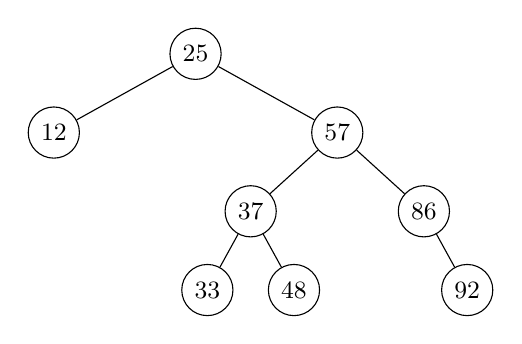
\begin{tikzpicture}[every node/.style={circle,draw,minimum size=6.5mm,inner sep=0pt,font=\small},
  level distance=10mm, level 1/.style={sibling distance=36mm}, level 2/.style={sibling distance=22mm},
  level 3/.style={sibling distance=11mm}]
\node {25}
  child {node {12}}
  child {node {57}
    child {node {37} child {node {33}} child {node {48}}}
    child {node {86} child[missing] child {node {92}}}};
\end{tikzpicture}
\end{center}
中序走訪 $12, 25, 33, 37, 48, 57, 86, 92$ 正好由小到大，確認是二元搜尋樹。 樹高 $4$（層數）。
\end{pastsoln}
